\documentclass[dvipsnames,tikz]{standalone}
\usepackage{amsmath}
\usepackage{arevmath}
\usepackage{xcolor}
\usepackage{tikz}
\usetikzlibrary{calc}
\usetikzlibrary{decorations.pathreplacing,calligraphy,3d}
\usepackage{tikz-3dplot} 

\tikzset{main/.style={thick, circle, color=black}}

\begin{document}
	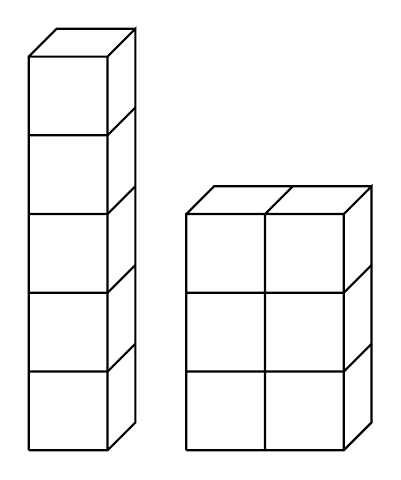
\begin{tikzpicture}[scale=1]
		\draw[main] (0,0) -- (1,0) --++(45:0.5) --++ (0,5) --++(225:0.5) --++(-1,0) --++(0,-5) (0,5) --++(45:0.5) --++(1,0) (1,0) --++(0,5);
		\draw[main] (0,1) --++(1,0) --++(45:0.5) (0,2) --++(1,0) --++(45:0.5) (0,3) --++(1,0) --++(45:0.5) (0,4) --++(1,0) --++(45:0.5);
		
		\begin{scope}[xshift=2cm]
			\draw[main] (0,0) --++(2,0) --++(45:0.5) --++ (0,3) --++(225:0.5) --++(-2,0) --++(0,-3) (0,3) --++(45:0.5) --++(2,0) (2,0) --++(0,3) ++(-1,0)++(45:0.5) --++(225:0.5) --++(0,-3);
			\draw[main] (0,1) --++(2,0)--++(45:0.5) (0,2) --++(2,0)--++(45:0.5);
		\end{scope}
	\end{tikzpicture}
\end{document}